\documentclass[journal, 10pt]{IEEEtran}

% =========================================================
% PACKAGES
% =========================================================
\usepackage{cite}
\usepackage{amsmath,amssymb,amsfonts}
\usepackage{algorithmic}
\usepackage{graphicx}
\usepackage{textcomp}
\usepackage{xcolor}
\usepackage{booktabs}
\usepackage{multirow}
\usepackage{hyperref}
\usepackage{tikz}
\usetikzlibrary{positioning, arrows.meta, fit, backgrounds}

\def\BibTeX{{\rm B\kern-.05em{\sc i\kern-.025em b}\kern-.08em
    T\kern-.1667em\lower.7ex\hbox{E}\kern-.125emX}}

\begin{document}

% =========================================================
% TITLE & AUTHORS
% =========================================================
\title{Pre-Mortem Feasibility Forecasting for New Software Requirements via Guardrailed LLM Parsing and Causal Intervention Simulation}

\author{
    \IEEEauthorblockN{Your Name\IEEEauthorrefmark{1}, Co-Author Name\IEEEauthorrefmark{2}} \\
    \IEEEauthorblockA{\IEEEauthorrefmark{1}Faculty of Information Technology, University of Engineering and Technology, \\
    Vietnam National University, Hanoi (VNU-UET), Vietnam \\
    Email: your.email@vnu.edu.vn}
}

\maketitle

% =========================================================
% ABSTRACT
% =========================================================
\begin{abstract}
When a new software requirement is proposed, engineering teams must judge
whether the existing microservice architecture can absorb the resulting
workload --- a question with no historical telemetry, since the feature
is not yet built.  We introduce a framework that combines a
\emph{Guardrailed LLM Parser}, translating natural-language requirements
into bounded causal interventions $do(X{=}x)$, with a
\emph{Dual-Path Structural Causal Model} that projects downstream resource
impact through a topology-adaptive, two-tier DAG.  Three symbolic
verification layers --- scope gate, entity grounding, and bounded
projection --- drive boundary-violation, hallucination, and
gateway-misdirection rates to exactly $0\%$ across 3 live-LLM repeats,
where unguarded baselines exceed $38\%$, $91\%$, and $100\%$ respectively.
On two RCAEval testbeds (Sock Shop, 7 services; Train Ticket, 28),
forecasting accuracy is competitive on the smaller topology but does
not transfer to the larger one; we argue this does not undermine the
contribution, which is a difference of \emph{kind}: an operator for
$do(x)$ feasibility queries that no regression baseline possesses.
\end{abstract}

\begin{IEEEkeywords}
Microservices, Requirements Feasibility Analysis, Causal Inference, Large Language Models, Multi-Agent System, Intervention Forecasting, AIOps.
\end{IEEEkeywords}

% =========================================================
% I. INTRODUCTION
% =========================================================
\section{Introduction}
\label{sec:introduction}

In microservice architectures, most new work during maintenance originates from an external \emph{requirement} --- a customer request, a product ticket, or a design document describing a feature that does not yet exist. Before committing engineering effort, teams must judge whether the architecture can absorb the workload this requirement will introduce --- a question that, by definition, has no historical telemetry to answer directly.

Current methodologies leave critical gaps. First, Causal RCA frameworks are retrospective, diagnosing incidents that have already occurred rather than ones an unbuilt feature might cause. Second, SCMs theoretically support counterfactual reasoning, yet applied research primarily solves $P(\text{Cause} \mid \text{Anomaly})$ rather than projecting the effect of a hypothetical requirement. Third, engineers lack a grounded way to turn natural-language requirements into quantitative workload assumptions, relying instead on heuristic estimation.

Our framework addresses these gaps by reframing microservice analysis toward prospective, requirement-level feasibility forecasting: given a natural-language requirement, project its downstream resource impact \emph{before} implementation, via Pearl's $do$-calculus. A $do(x)$ query and a more accurate point forecast answer fundamentally different questions (Section~\ref{sec:background}); consequently, the contribution is the $do(x)$ operator itself, not forecast accuracy.

\textbf{Scope.} We bound ``new requirement'' to features approximable by an existing calibration archetype within the target system's request taxonomy (Section~\ref{sec:methodology}) --- e.g., a new promotion mechanic is treated as a variant of an existing checkout-discount archetype. A requirement matching no known archetype is out of scope for a numeric verdict; Section~\ref{sec:discussion} discusses how the implementation handles this case.

Our main contributions are:
\begin{enumerate}
    \item \textbf{Grounded Parameter Estimation via LLM-Modulo:} A Parser Agent bounded by a three-layer symbolic verification architecture --- \emph{(i)} a \textbf{Scope Gate} implementing selective abstention, \emph{(ii)} an \textbf{Entity Grounding} layer enforcing graph-membership invariants, and \emph{(iii)} a \textbf{Bounded Projection} operator $\Pi$ clamping numeric deltas to empirically anchored safety envelopes --- drives three observed failure modes to exactly $0\%$ across 3 live-LLM repeats (Section~\ref{sec:results}).
    \item \textbf{Modeling Cascade Attenuation:} A topology-adaptive, multi-tier hierarchical SCM ($4{\times}|V|$ nodes, fit per-testbed) disentangles network-layer propagation from hardware-layer consumption, enabling forward interventional attribution via the Shapley-over-DAG machinery of Budhathoki et al.\ \cite{budhathoki2022rootcause}; its faithfulness at scale is treated as future work (Section~\ref{sec:future-work}).
    \item \textbf{Domain-Aware Causal Mechanisms:} A queueing-inspired regressor models non-linear latency bottlenecks within the SCM's structural equations, evaluated both in- and out-of-distribution.
    \item \textbf{Cross-Topology Evaluation:} The full pipeline is evaluated on two topologies of substantially different scale (7 vs.\ 28 services), reporting where conclusions do and do not transfer.
\end{enumerate}

% =========================================================
% II. BACKGROUND & RELATED WORK
% =========================================================
\section{Background and Related Work}
\label{sec:background}

\subsection{From Retrospective RCA to Prospective Forecasting}
Traditional machine learning fits an association between $X$ and $Y$ within the observed distribution, not a mechanism that holds once $X$ is deliberately changed. Pearl's SCM \cite{pearl2009causality} resolves this via the $do$-calculus operator: the Truncated Factorization Theorem states that for an intervention $do(X_i = x_i^*)$,
\begin{equation}
P(x_1,\dots,x_n \mid do(X_i{=}x_i^*)) = \prod_{j\neq i} P(x_j \mid pa_j)\Big|_{X_i = x_i^*},
\end{equation}
i.e.\ the interventional distribution is built from the \emph{same} conditional mechanisms $P(x_j\mid pa_j)$ with the edges into $X_i$ severed rather than conditioned on. A regression baseline has no such operator: its estimate $\hat y = h(x)$ need not equal $\mathbb{E}[Y \mid do(X{=}x)]$ under confounding, because the associational and interventional quantities are provably distinct \cite{pearl2009causality}. With a fitted SCM, answering a $do(x)$ query reduces to forward simulation --- computationally trivial --- whose completeness Huang and Valtorta established for Pearl's three inference rules \cite{huang2006complete}. This establishes the \emph{well-definedness} of $do(x)$, not the empirical accuracy of our fitted mechanisms; the latter is reported in RQ1--RQ2, including where unfavorable.

Existing SCM-based microservice diagnostics apply this structure \emph{retrospectively}: Budhathoki et al.\ \cite{budhathoki2022rootcause} attribute an already-observed outlier to upstream root causes via Shapley values over a causal graph --- the same mechanism DoWhy-GCM \cite{blobaum2024dowhy} exposes as \texttt{attribute\_anomalies}. We run this machinery in the opposite, \emph{prospective} direction: given a hypothetical $do(\text{Workload}{=}w)$, we ask which downstream nodes it would push into outlier territory before the workload is applied. Formally, let $\tilde x := \mathbb{E}[X \mid do(\text{Workload}{=}w)]$ be obtained by forward simulation through the fitted DAG (Section~\ref{sec:workload-propagation}); the Shapley decomposition $S(\tilde x) = \sum_j c^{Sh}_{\tilde x}(j)$ of \cite{budhathoki2022rootcause} applies identically, licensed by the modularity property \cite{blobaum2024dowhy}: $do(X_k{=}x_k^*)$ replaces only the mechanism at node $k$, leaving $N_{j\neq k}$ jointly independent regardless of whether $x_k^*$ was measured or hypothesized. Its faithfulness at scale remains untested (Section~\ref{sec:threats}).

\subsection{Neuro-Symbolic AI and LLM Verification}
Recent studies highlight that while LLMs possess exceptional semantic reasoning, they exhibit severe deficiencies in deterministic planning \cite{kambhampati2024}. Following the LLM-Modulo and symbolic-feedback frameworks, we position the LLM strictly as a candidate generator, relying on external architectural guardrails to enforce correctness and topological constraints. Our multi-agent orchestration follows the ReAct paradigm of interleaved reasoning and tool-acting \cite{yao2022react}.

\subsection{Benchmarks and Statistical Comparison}
We evaluate on RCAEval \cite{pham2024rcaeval}, a public microservice RCA benchmark providing fault-injected telemetry for both Sock Shop and Train Ticket topologies. For comparing multiple models across datasets we follow the non-parametric testing methodology of Demšar \cite{demsar2006}, using paired Wilcoxon signed-rank and Friedman tests rather than parametric tests, given the small number of independent services per system.

% =========================================================
% III. METHODOLOGY
% =========================================================
\section{Methodology}
\label{sec:methodology}

\textbf{Notation.} Let $\mathcal{G} = (V, E)$ denote the dependency graph, where $V = V_W \cup V_R$ partitions into workload and resource nodes. For node $j$, $PA_j$ denotes its parent set in $\mathcal{G}$ and $N_j$ its exogenous noise term.

\subsection{System Architecture Overview}
The system is a four-node LangGraph state machine (Fig.~\ref{fig:architecture}) executed sequentially per requirement: the Parser Agent (Section~\ref{sec:parser-agent}) turns text into a bounded intervention $do(X{=}x)$; the Architecture Agent performs a breadth-first traversal from the injection gateway to determine the blast radius of affected services; the Capacity Agent projects downstream resource consumption along two paths -- a fast per-service bivariate SCM and an accurate, topology-adaptive global DAG propagating through both the cross-service workload tier and the local resource-consumption tier (Section~\ref{sec:workload-propagation}); and an LLM synthesizes the projected metrics and a self-critique (``Devil's Advocate'') pass into a natural-language \texttt{FeasibilityReport}. Only the first and third nodes involve the causal/LLM machinery evaluated in Section~\ref{sec:results}; the second is a deterministic graph traversal and the fourth is not evaluated quantitatively.

\begin{figure}[t]
\centering
\resizebox{\linewidth}{!}{%
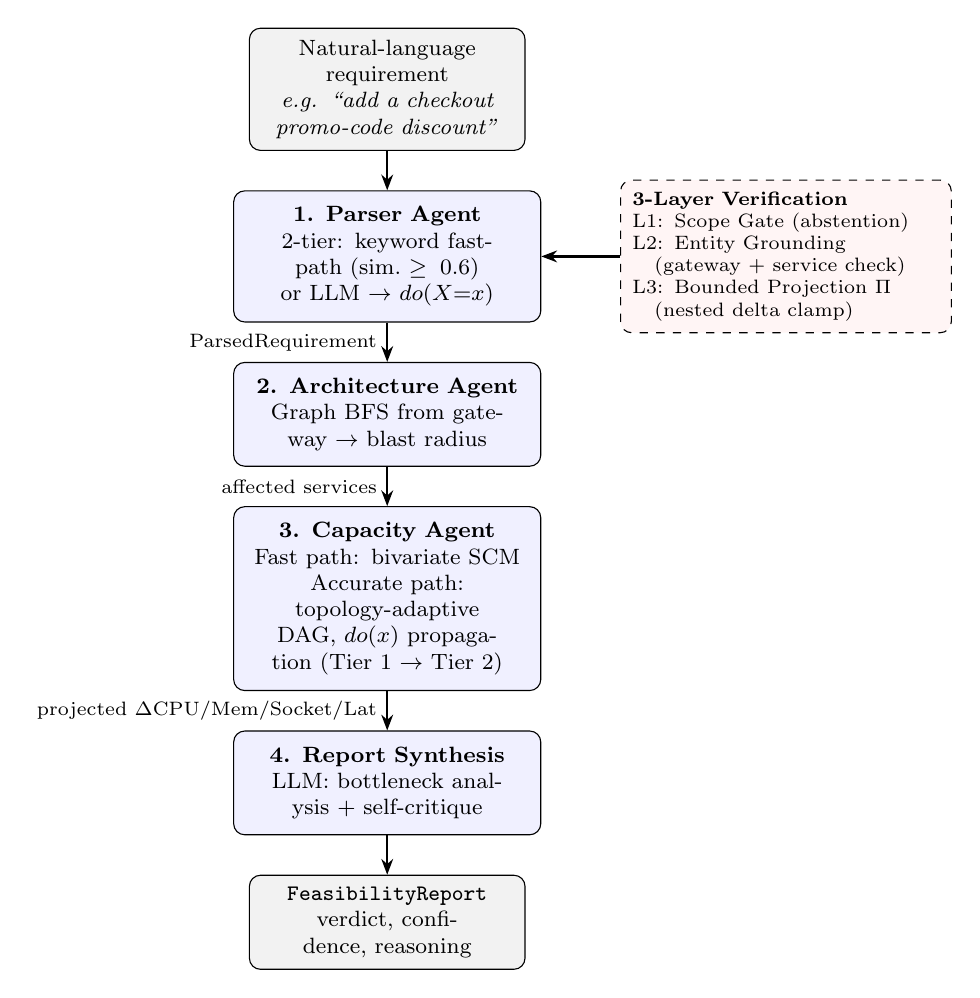
\begin{tikzpicture}[
    font=\footnotesize,
    node distance = 5mm and 8mm,
    stage/.style = {draw, rounded corners, fill=blue!6, align=center, text width=3.5cm, minimum height=10mm, inner sep=2mm},
    io/.style = {draw, rounded corners, fill=gray!10, align=center, text width=3.2cm, minimum height=6mm, inner sep=1.5mm},
    guardbox/.style = {draw, dashed, rounded corners, fill=red!4, align=left, text width=3.9cm, inner sep=1.5mm, font=\scriptsize},
    arrow/.style = {-{Stealth[length=2mm]}, thick}
]
    \node[io] (input) {Natural-language requirement\\ \emph{e.g. ``add a checkout promo-code discount''}};
    \node[stage, below=of input] (parser) {\textbf{1. Parser Agent}\\ \footnotesize 2-tier: keyword fast-path (sim.\ $\geq0.6$) or LLM $\rightarrow$ $do(X{=}x)$};
    \node[guardbox, right=of parser, xshift=2mm] (guards) {\textbf{3-Layer Verification}\\ L1: Scope Gate (abstention)\\ L2: Entity Grounding\\ \quad (gateway + service check)\\ L3: Bounded Projection $\Pi$\\ \quad (nested delta clamp)};
    \node[stage, below=of parser] (arch) {\textbf{2. Architecture Agent}\\ \footnotesize Graph BFS from gateway $\rightarrow$ blast radius};
    \node[stage, below=of arch] (capacity) {\textbf{3. Capacity Agent}\\ \footnotesize Fast path: bivariate SCM\\ Accurate path: topology-adaptive DAG, $do(x)$ propagation (Tier 1 $\rightarrow$ Tier 2)};
    \node[stage, below=of capacity] (report) {\textbf{4. Report Synthesis}\\ \footnotesize LLM: bottleneck analysis + self-critique};
    \node[io, below=of report] (output) {\texttt{FeasibilityReport}\\ verdict, confidence, reasoning};

    \draw[arrow] (input) -- (parser);
    \draw[arrow] (parser) -- (arch) node[midway, left, font=\scriptsize] {ParsedRequirement};
    \draw[arrow] (guards.west) -- (parser.east);
    \draw[arrow] (arch) -- (capacity) node[midway, left, font=\scriptsize] {affected services};
    \draw[arrow] (capacity) -- (report) node[midway, left, font=\scriptsize] {projected $\Delta$CPU/Mem/Socket/Lat};
    \draw[arrow] (report) -- (output);
\end{tikzpicture}%
}
\caption{System pipeline: a four-node LangGraph state machine from natural-language requirement to feasibility verdict. Only nodes 1 and 3 (solid arrows into causal/LLM machinery) are quantitatively evaluated in Section~\ref{sec:results}; node 2 is a deterministic graph traversal and node 4 is unevaluated text synthesis.}
\label{fig:architecture}
\end{figure}

\subsection{Parser Agent: Semantic Bridge and Three-Layer Verification}
\label{sec:parser-agent}
The Parser Agent translates natural language into a quantitative intervention vector $do(X=x)$. It follows a two-tier strategy: a deterministic keyword-similarity match against an empirical calibration table is attempted first (bypassing the LLM entirely when similarity $\geq \tau$, with $\tau = 0.6$); otherwise the LLM is invoked to propose a request type, affected services, and a bounded adjustment. The same threshold $\tau$ also controls, within the LLM branch, whether the LLM's proposed adjustment is used or zeroed (forcing the calibration anchor unmodified when match confidence is low). Since sweeping $\tau \in [0.3, 0.8]$ on the RQ3 test set left all safety metrics (PBVR, SHR, Anchor MAE) completely unchanged — only the fast-path bypass rate shifted — we treat $\tau$ as a cost--accuracy design parameter rather than a safety mechanism, and do not count it among the verification layers below.

In both branches, the output passes through a \textbf{three-layer symbolic verification architecture} before being returned. Following the LLM-Modulo separation of concerns \cite{kambhampati2024}, the LLM is treated strictly as a non-deterministic candidate generator $L$, and a deterministic, sound verifier enforces all safety properties independently of $L$'s reliability. The three layers are organized by their distinct mathematical purpose — selective abstention, graph-membership enforcement, and interval projection — rather than enumerated as a flat list, and each targets one category of failure mode we observed the unguarded LLM exhibit.

\subsubsection{Layer 1: Scope Gate (Selective Abstention)}
\label{sec:scope-gate}
The LLM branch is explicitly instructed to always select the closest-matching known request type rather than decline (Section~\ref{sec:edge-of-scope}), so after it returns a choice we independently recompute keyword similarity against \emph{that chosen type's own} keyword list. Zero overlap for both the rule-based guess and the LLM's own selection sets confidence to \textsc{refused} and flags \texttt{is\_out\_of\_scope}; the report-generation node short-circuits to an explicit refusal report instead of letting the downstream LLM synthesize a confident verdict around a fallback number. This layer implements \emph{selective abstention} rather than projection -- a qualitatively different behavior from Layers 2 and 3, which correct invalid candidates rather than refuse them.

One limitation: the zero-keyword-overlap criterion is coarse. A requirement that shares one incidental keyword with an unrelated archetype would not trigger it, so this is a floor on refusal recall, not a complete taxonomy-membership detector.

\subsubsection{Layer 2: Entity Grounding (Graph-Membership Invariants)}
\label{sec:entity-grounding}
This layer enforces that every entity proposed by the LLM corresponds to a real node in the topology graph $\mathcal{G}$ — a deterministic set-membership check with no free parameter.
\begin{itemize}
    \item \textbf{Gateway Invariance:} the injection point $do(x)$ must be applied at a node with in-degree $= 0$; if the LLM proposes an internal node, the system falls back to the nearest valid gateway and downgrades confidence to \textsc{low}. On RQ3's 50-prompt benchmark the LLM's own \texttt{injection\_service} proposal was always correct (\texttt{front-end}, unanimously across 150 live calls); an 18-prompt adversarial set describing plausible backend/async work induced a non-gateway proposal on \emph{every} prompt, and the fallback corrected all $18/18$ -- demonstrating \emph{rejection} on this single-gateway topology, not \emph{disambiguation} between two valid gateways, which requires a topology this one lacks (Section~\ref{sec:threats}).
    \item \textbf{Service Existence Filter:} discards any proposed \texttt{core\_services} entry that does not correspond to a real node in $\mathcal{G}$, preventing hallucinated services from propagating downstream.
\end{itemize}

\subsubsection{Layer 3: Bounded Projection $\Pi$ (Empirically Anchored Clamping)}
\label{sec:bounded-projection}
This layer constrains how far the LLM's numeric proposal may deviate from the empirical calibration table. It is the only layer with hand-set numeric thresholds, and Section~\ref{sec:discussion} reports how well each is empirically justified. In the implementation, both clamps are applied by a single function (\texttt{\_guard\_delta}) in one pass — a nested bound rather than two independent mechanisms — but we describe them separately because their empirical status differs:
\begin{itemize}
    \item \textbf{Outer Clamp (Physical Delta Bound):} clamps the proposed workload delta to $[5\%, 50\%]$. This range sits at a knee: replaying the 300 raw, unguarded LLM proposals from RQ3's B1/B2 baselines (up to $50{,}000\%$) against candidate bounds, tightening to $[10,30]$ nearly doubles the flagged-violation rate ($26.3\%\to47.0\%$), while loosening to $[1,100]$ barely helps ($26.3\%\to21.3\%$) -- the excluded tail is pathologically extreme, not borderline.
    \item \textbf{Inner Clamp (Adjustment Bound):} restricts the LLM's fine-tuning of the calibration anchor to $\pm 10\%$, before the outer clamp applies; violations fall back to the unadjusted anchor. Its $0\%$ RQ3 trigger rate held even with the $[-10,10]$ instruction removed from the prompt (3 repeats, $0/141$), ruling out circularity. A 12-prompt adversarial set (two archetypes $\times$ six manipulation strategies: direct override, extreme-narrative framing, fabricated authority, forced step-by-step reasoning, urgency framing, roleplay override) pushed raw adjustments as high as $+500\%$ and triggered the clamp on $33/36$ ($91.7\%$, every strategy but roleplay). The inner clamp is therefore genuinely load-bearing: inert against benign prompts, but the only mechanism standing between a manipulated proposal and a $500\%$ delta reaching the SCM.
\end{itemize}

\textbf{Formalization.} Let $L : \Sigma^* \to T \times \mathbb{R} \times 2^V$ be the LLM's candidate generator, mapping a raw requirement $r$ to a proposed $(t, \delta, S)$ — request type, workload delta, and core-service set. Layers 2 and 3 compose into a single deterministic \emph{bounded projection operator} $\Pi$ applied to every candidate regardless of $L$'s output distribution:
\begin{equation}
\Pi(t,\delta,S) = \big(\textsc{Gw}(\text{inj}),\ \textsc{Clamp}_{[5,50]}(\delta_{\text{anchor}} + \textsc{Clamp}_{[-10,10]}(\text{adj})),\ S \cap V\big),
\end{equation}
with $\textsc{Gw}(v) = v$ if $\text{in-deg}(v)=0$, else the nearest valid gateway; $\textsc{Clamp}_{[a,b]}(x) = \max(a,\min(b,x))$. Because $\Pi$ is total and deterministic, its output guarantees -- valid gateway, $\delta \in [5,50]$, $S \subseteq V$ -- hold for every input regardless of whether $L$ hallucinates. Layer 1 differs qualitatively: rather than projecting an out-of-range candidate back into a valid one, it detects when no projection can be trusted at all and substitutes an explicit refusal for a numeric verdict.

The dependency topology is separately verified acyclic at graph-construction time (a structural precondition, not a per-request layer). A hard $[0,100]$ clamp on predicted resource values, considered in early design, was not implemented; Section~\ref{sec:extrapolation} discusses the failure mode this gap causes and how we mitigate it at the causal-mechanism level instead. The pipeline evaluated here supports only single-intervention queries -- no additive-shift rule for simultaneous ancestor--descendant interventions exists.

\subsection{Workload Propagation and Causal Simulation}
\label{sec:workload-propagation}
The Capacity Agent's accurate path models degradation using a two-tier DAG (28 nodes on Sock Shop; a 112-node instance of the same construction has also been fit on Train Ticket) with DoWhy's Additive Noise Model framework. The node set is partitioned $V = V_W \cup V_R$ into cross-service workload nodes and local resource nodes, with edges restricted to two kinds by default:
\begin{align}
\text{Tier 1 (workload):} \quad & W_j = f_j(PA_{W_j}) + N_{W_j}, \ PA_{W_j}\subseteq V_W, \\
\text{Tier 2 (resource):} \quad & R_j = g_j(PA_{R_j}) + N_{R_j}, \ PA_{R_j}\subseteq \{W_j\}\cup V_R,
\end{align}
i.e.\ each resource node $R_j$ (CPU, memory, latency) has its own service's workload $W_j$ as a parent, and \emph{by default} no other: no $R \to R$ or $R \to W$ edges. This default is what makes the per-node Shapley decomposition of Section~\ref{sec:background} \emph{potentially} interpretable as which tier is responsible for a projected change, not merely which node — whether this holds up under a controlled, ground-truth check is evaluated separately \cite{ourxaipaper} rather than assumed here. It is not exceptionless: Section~\ref{sec:backpressure-edge} adds $R\to R$ edges -- one or more caller services' own CPU as additional parents of a callee's CPU -- on a small, individually-validated set of nodes ($3$ of $21$ CPU/memory nodes on Sock Shop, $20$ of $84$ on Train Ticket, some receiving as many as five simultaneous caller-CPU parents), which is exactly why we flag it there as narrowing the tier-decomposition's clean interpretability on precisely those nodes, not only as an accuracy change.

Resource-consumption mechanisms $g_j$ (CPU, memory) are fit as $g_j(w) = \boldsymbol{\beta}^\top w + \beta_0$ with coefficients constrained to $\boldsymbol{\beta}^* = \operatorname*{argmin}_{\boldsymbol{\beta}\geq \mathbf{0}} \lVert \mathbf{y} - X\boldsymbol{\beta}\rVert_2^2$ (non-negative least squares), which guarantees $\partial g_j/\partial w \geq 0$ and enforces a monotonically non-decreasing response to workload by construction (Section~\ref{sec:extrapolation}) — applied uniformly to both tiers, not only Tier 2. Latency mechanisms instead use a queueing-inspired regressor with feature transform
\begin{equation}
\phi(w) := \frac{w}{c-w}, \qquad c \approx 1.5 \max(W_{\text{train}}),
\end{equation}
fit as $R^{\text{Latency}}_j = \beta\,\phi(W_j) + \beta_0$, $\beta\geq 0$; as $w \to c^-$, $\phi(w)\to\infty$, approximating the heavy-traffic behavior $\rho/(1-\rho)$ of an M/M/1 queue as utilization approaches capacity $c$ \cite{kingman1961}, rather than a closed-form derivation from queueing theory.

\textbf{Post-Simulation Uncertainty Annotation.} The three-layer verification (Section~\ref{sec:parser-agent}) bounds the \emph{input} intervention delta to $[5\%,50\%]$, but a downstream node reached through Tier-1/Tier-2 propagation can still land outside \emph{its own} training envelope even when the injection delta is legal. Sweeping the full legal range on both testbeds and comparing every downstream node's projected mean against its own training-distribution percentiles, $16.7\%$ of (node, delta) pairs on Sock Shop fall outside the P90 band ($3.7\%$ already at $5\%$, rising to $25.9\%$ at $50\%$), versus only $0.4\%$ on Train Ticket -- the risk is real but topology-dependent. After each simulation, every downstream node's projected mean is therefore classified against its own training percentiles (\textsc{high}$\leq P_{90}$; \textsc{medium}$\leq P_{95}$; \textsc{low}$\leq\max(P_{99}, 2\times\max_{\text{train}})$; \textsc{very\_low} beyond that), and \texttt{generate\_report\_node} deterministically appends an extrapolation-risk caveat, naming the flagged nodes, whenever the worst confidence is \textsc{low} or \textsc{very\_low} -- attaching a caveat to a still-legitimate verdict rather than replacing it, the same code-level-guarantee design as the Scope Gate but for a familiar request type pushed to an unusual magnitude, rather than one matching no archetype at all.

We present this transparently as an \emph{annotation}, not a verification layer: against RQ3's 150 real cases, it fires on $80\%$ of ordinary, in-taxonomy cases -- far above the $16.7\%$ the uniform sweep suggests -- and $147/150$ are driven by one node, \texttt{catalogue\_cpu}, whose heavily right-skewed training distribution (P95$=0.21$, max$=49.0$) makes its band narrow enough that a typical delta exceeds it. This annotation therefore has low specificity as currently calibrated: a caveat on 4 out of 5 reports is not one a user can act on selectively. We do not attempt an ad hoc per-node recalibration, since doing so without a principled methodology risks trading one unvalidated threshold for another; we report the finding and leave recalibration to future work (Section~\ref{sec:future-work}).

% =========================================================
% IV. EXPERIMENTAL SETUP
% =========================================================
\section{Experimental Setup}
\label{sec:setup}

\subsection{Datasets and Testbed}
We evaluate our framework on RCAEval \cite{pham2024rcaeval}: \textbf{Sock Shop} (7 microservices, 90 fault-injection scenarios: 30 fault types $\times$ 3 runs) and \textbf{Train Ticket} (28 microservices, up to 384 metric columns, the same 90-scenario protocol scale: 5 target services $\times$ 6 fault types $\times$ 3 runs). Both share the same telemetry schema (workload, CPU, memory, socket count, $p50$/$p90$ latency, with an explicit fault-injection timestamp); RQ1/RQ2 evaluate CPU, Memory, and Socket on both systems (Tables~\ref{tab:rq1}, \ref{tab:rq1-gt}), excluding Latency from the 4-model comparison because standard regressors do not model its saturating behavior (Section~\ref{sec:workload-propagation}), not from a schema difference. We report results per-system rather than pooled, to avoid obscuring topology-specific variation.

\subsection{Baselines for Comparison}
\begin{itemize}
    \item \textbf{(B0) Rule-Only Parser:} a deterministic keyword-matching classifier with no LLM and no learned adjustment, used as the accuracy floor for requirement parsing.
    \item \textbf{(B1) Unguarded Zero-Shot LLM:} the same live LLM backend as our proposed parser, prompted directly with no calibration table and no runtime guards.
    \item \textbf{(B2) Unguarded Few-Shot LLM:} as B1, but with the system topology and calibration table given as in-context examples, still without any runtime guard.
    \item \textbf{(B3) Non-Causal Regression Baselines:} Linear Regression, Gradient Boosting Regression, and a Gaussian Process Regressor, trained and evaluated under the identical out-of-distribution protocol as the SCM (Section~\ref{sec:results}), used to test whether causal structure yields an accuracy advantage over standard regressors.
    \item \textbf{(B4) Uniform Delta Injection:} a naive propagation baseline that assumes every downstream service's workload changes by exactly the same percentage as the injected upstream delta, bypassing the dependency-graph propagation entirely.
\end{itemize}

\subsection{Evaluation Metrics}
We measure forecasting accuracy using MAPE, RMSE, and $R^2$, computed at full test-set resolution (i.e., on every held-out point rather than on quantile-bucket averages, which we found to substantially understate error \textemdash Section~\ref{sec:results}). For the Parser Agent we additionally report the Physical Boundary Violation Rate (PBVR), Service Hallucination Rate (SHR), and Gateway Misdirection Rate (GMR), plus mean end-to-end inference latency and the fraction of requests resolved without an LLM call (fast-path bypass rate).

% =========================================================
% V. RESULTS AND EVALUATION
% =========================================================
\section{Results and Evaluation}
\label{sec:results}

We organize results around five research questions. RQ1--RQ2 evaluate forecasting accuracy and compare the SCM against non-causal regressors. RQ3 evaluates Parser reliability under the three-layer verification architecture. RQ4 tests graph-based propagation against a uniform-delta baseline, and RQ5 measures multi-agent coordination overhead.

\subsection{RQ1: Out-of-Distribution Forecasting Accuracy, Per System}
We train on the lowest 67\% of observed workload and test on the highest 33\%, forcing genuine extrapolation, and report full-resolution error (every held-out point, via the closed-form additive-noise-model prediction $\mathbb{E}[\text{Target} \mid do(\text{Workload}=w)]$, avoiding Monte Carlo sampling) alongside a legacy 8-bucket quantile average, since bucket-averaging understates error on the large majority of pairs. The mechanism fit here is the same non-negative-coefficient linear model (Section~\ref{sec:extrapolation}) deployed in the bivariate fast path: we report the accuracy this deployed mechanism achieves, trading full-resolution point-accuracy on CPU/Socket for the sign-correctness guarantee it exists for.

\begin{table}[h]
\centering
\caption{Full-resolution SCM forecasting error, per system (mean $\pm$ range across services)}
\label{tab:rq1}
\begin{tabular}{lccc}
\toprule
System & Metric & MAPE mean (range) \% & $n$ services \\
\midrule
Sock Shop   & CPU    & 46.8 (10.2--82.0) & 7 \\
Sock Shop   & Memory & 3.9 (1.3--7.9)    & 7 \\
Sock Shop   & Socket & 26.7 (8.3--60.8)  & 7 \\
Train Ticket & CPU    & 68.6 (8.9--109.3) & 28 \\
Train Ticket & Memory & 2.3 (0.9--4.5)    & 28 \\
Train Ticket & Socket & 15.9 (5.5--39.9)  & 28 \\
\bottomrule
\end{tabular}
\end{table}

As an independent check that does not reuse the accuracy-benchmark's train/test split, we additionally match SCM predictions directly against real measured values across all fault-injection scenarios, splitting each scenario chronologically (70\%/30\%) rather than pooling across scenarios (Table~\ref{tab:rq1-gt}).

\begin{table}[h]
\centering
\caption{Ground-truth direct match (no bucketing, per-scenario chronological split)}
\label{tab:rq1-gt}
\resizebox{\linewidth}{!}{%
\begin{tabular}{llccc}
\toprule
System & Metric & $n$ points & Mean \%err & Median \%err \\
\midrule
Sock Shop    & CPU     & 136{,}496 & 33.5 & 9.1 \\
Sock Shop    & Memory  & 136{,}674 & 2.3  & 0.4 \\
Sock Shop    & Socket  & 136{,}674 & 5.8  & 2.8 \\
Sock Shop    & Latency $p50$ & 134{,}625 & 9.9 & 2.0 \\
Train Ticket & CPU     & 528{,}388 & 49.8 & 23.2 \\
Train Ticket & Memory  & 528{,}518 & 0.7  & 0.2 \\
Train Ticket & Socket  & 528{,}518 & 8.4  & 5.5 \\
\bottomrule
\end{tabular}%
}
\end{table}

In both systems, mean error exceeds the median by $3{\times}$--$4{\times}$ (e.g., Sock Shop CPU: $33.5$ vs.\ $9.1$), reflecting a right-skewed distribution: most points forecast well, but a minority under active fault injection incur large errors. On Sock Shop, full-resolution $R^2$ is negative for 16 of 21 pairs (20 of 21 under bucket-averaging); the SCM does not explain held-out variance better than a mean predictor here, even where MAPE is acceptable for capacity planning.

\subsection{RQ1 Follow-Up: A Validated Backpressure Extension}
\label{sec:backpressure-edge}
The Global DAG's Tier-2 mechanism (Section~\ref{sec:workload-propagation}) is extended, on a small validated node subset, with a second parent: a directly-calling service's own CPU, capturing synchronous backpressure a callee's request count does not (cluster-wide contention and target-smoothing were tested and ruled out). This parent is \emph{added}, never substituted for the callee's own workload -- a caller-CPU-only mechanism fits the observational data almost as well but predicts \emph{zero} response to a requirement injected directly at the callee, an interventional failure the $do(x)$-versus-$P(Y\mid X)$ distinction (Section~\ref{sec:background}) predicts and observational fit alone cannot reveal.

Validated against held-out data under RQ1's own OOD protocol and the extrapolation-sign sweep of Section~\ref{sec:extrapolation}, rather than the in-sample fit that surfaced it: on Sock Shop, the extension covers $3$ of $21$ CPU/memory nodes (\texttt{orders}$\to$\{\texttt{carts},\texttt{shipping}\}, \texttt{front-end}$\to$\texttt{user}) -- mean full-resolution MAPE falls $48.4\%\to40.3\%$, mean $R^2$ turns positive ($-0.030\to0.084$), threshold-crossing F1 improves $\times 3.9$ ($0.103\to0.401$), and total sign-inversions across $+5\%$--$+300\%$ fall $30\to24$, correcting two pre-existing physically-implausible cases outright (\texttt{orders} at $+150\%$ no longer predicts a \emph{decrease} in \texttt{carts\_cpu} or a flat \texttt{shipping\_cpu}). On Train Ticket, the same protocol applied to its real \texttt{REST\_CALL} topology covers $20$ of $84$ CPU nodes (several, e.g.\ \texttt{ts-station-service}, with up to five simultaneous caller-CPU parents fit jointly rather than one at a time) -- MAPE, $R^2$, and F1 improve on all $20$ nodes with no exception (mean MAPE $71.1\%\to44.9\%$; mean $R^2$ $-0.15\to0.32$; mean F1 $0.176\to0.592$). Two services, \texttt{catalogue} and \texttt{payment}, remain unexplained by this or any covariate we tested, consistent with request-independent background work.

Total sign-inversions on Train Ticket fall overall ($35\to26$) but rise from $8$ to $11$ ($+37\%$) at the single most extreme delta ($+300\%$), at nodes mostly several hops from the new edges --- consistent with the linear-positive mechanism's pre-existing extrapolation fragility (Section~\ref{sec:extrapolation}) being amplified by a denser graph rather than a defect specific to these edges. We deployed the extension on both testbeds: a $23/23$-node improvement in accuracy outweighs a cost confined to a delta band already treated as directional rather than validated. The Global DAG now has $32$ edges (from $29$) on Sock Shop and $200$ (from $150$) on Train Ticket, verified through the same production method (\texttt{CapacityAgent.simulate\_intervention}) the orchestrator calls.

\subsection{RQ2: Does Causal Structure Improve Accuracy Over Non-Causal Regressors?}
We compare the SCM against B3 (Linear Regression, Gradient Boosting, Gaussian Process) under the identical protocol, using paired Wilcoxon and Friedman tests on full-resolution MAPE, computed \emph{separately per metric} (CPU, Memory, Socket use incompatible units and cannot be pooled into a single RMSE-based test without inflating apparent significance).

On \textbf{Sock Shop} ($n=21$ service--metric pairs), the SCM is statistically significantly more accurate than Linear Regression when pooled across metrics ($p=0.0137$, median $\Delta = -0.94$ MAPE points, SCM lower), but is statistically indistinguishable from Gradient Boosting ($p=0.812$) and Gaussian Process ($p=0.421$). By win count, the SCM ties for first place (7/21 service--metric combinations), alongside Gaussian Process (7/21), ahead of Gradient Boosting (6/21) and Linear Regression (1/21).

On \textbf{Train Ticket} ($n=84$ pairs across CPU, Memory, Socket -- $4\times$ larger than Sock Shop), the result does \emph{not} replicate in the SCM's favor: it wins only 12/84, the fewest of the four models (Gaussian Process 30/84, Gradient Boosting 23/84, Linear Regression 19/84). Pooled, the SCM is significantly more accurate than Linear Regression here too ($p<0.0001$, median $\Delta=-0.12$; driven by a large CPU effect, $\Delta=-15.66$, $p=0.0001$); against Gaussian Process the pooled comparison is not significant ($p=0.432$), masking opposite-signed per-metric effects: significantly \emph{less} accurate on CPU ($\Delta=+4.90$, $p=0.0095$), significantly \emph{more} on Memory ($\Delta=-0.025$, $p=0.020$, negligible in absolute terms), Socket not significant; against Gradient Boosting the SCM remains indistinguishable, pooled and per-metric ($p=0.156$). The recurring pattern -- beating the simplest baseline while not separating from the two more flexible ones -- is consistent with the SCM's own mechanisms being close to linear-regression-equivalent in structure (Section~\ref{sec:workload-propagation}); pooling across metrics can mask offsetting per-metric effects, which we flag rather than report only the most favorable $p$-value.

\textbf{We do not conclude that SCM point-accuracy is superior to standard regressors.} The advantage on Sock Shop does not transfer to Train Ticket, and we interpret this as evidence that the framework's value rests on its unique capability --- supporting $do(x)$ intervention queries that regression baselines cannot answer at all --- rather than on raw predictive accuracy. A regression baseline returns a scalar $\hat y$ with no causal graph to decompose; the SCM's projection can in principle be attributed to the responsible service and tier via Shapley decomposition (Section~\ref{sec:background}), though this attribution mechanism is implemented but not yet validated for faithfulness (Section~\ref{sec:threats}).

\subsection{RQ3: Do Guardrails Improve LLM Calibration? (Live LLM Evaluation)}
We evaluate 50 hand-authored requirement prompts (In-Distribution, Complex Multi-Hop, Subtle Read-Only, and Adversarial subsets) against four parser configurations, using a live LLM backend (\texttt{gemini-flash-lite-latest}) rather than a scripted stand-in, so that failure modes reflect genuine model behavior rather than an experimenter-authored fixture.

\begin{table}[h]
\centering
\caption{Parser reliability, live LLM, 50 prompts, mean $\pm$ std over 3 independent repeats}
\label{tab:rq3}
\resizebox{\linewidth}{!}{%
\begin{tabular}{lcccc}
\toprule
Configuration & PBVR & SHR & GMR & Anchor MAE \\
\midrule
Unguarded Zero-Shot (B1) & 38.0$\pm$2.0\% & 91.3$\pm$1.2\% & 100.0$\pm$0.0\% & 844.6$\pm$568.2\% \\
Unguarded Few-Shot (B2)  & 14.7$\pm$1.2\% & 2.0$\pm$0.0\%  & 84.7$\pm$1.2\%  & 38.6$\pm$0.2\%  \\
Rule-Only (B0)           & 0.0$\pm$0.0\%  & 0.0$\pm$0.0\%  & 0.0$\pm$0.0\%   & 2.8$\pm$0.0\%   \\
\textbf{Guarded (Ours)}  & \textbf{0.0$\pm$0.0\%} & \textbf{0.0$\pm$0.0\%} & \textbf{0.0$\pm$0.0\%} & \textbf{2.2$\pm$0.2\%} \\
\bottomrule
\end{tabular}%
}
\end{table}

Across 3 independent live-LLM repeats (temperature 0.2), the unconstrained LLM (B1) misdirects the injection point away from the gateway on \emph{every} prompt (GMR $=100.0\pm0.0\%$), hallucinates services on $91.3\pm1.2\%$ of prompts (SHR), and violates a physical bound on $38.0\pm2.0\%$ (PBVR); these compound into a mean Anchor MAE of $844.6\pm568.2\%$ (range $188.5$--$1173.4\%$). This mean is right-skewed, as in RQ1: the per-repeat median is far lower ($22.8$--$30.0\%$), inflated by only 2--3 of 50 prompts per repeat going wildly out of bound -- most strikingly a ``DDoS via millions of fake promo-code requests'' prompt answered with a literal $50{,}000\%$ delta. We flag the instability explicitly: an unguarded LLM's output is not merely inaccurate on average, it is unstable run-to-run, which a single-repetition evaluation cannot reveal. In-context calibration (B2: few-shot topology and calibration table, still no runtime guard) closes most of the gap on two metrics (SHR $\to2.0\pm0.0\%$, Anchor MAE $\to38.6\pm0.2\%$) but leaves GMR at $84.7\pm1.2\%$ and PBVR at $14.7\pm1.2\%$: better prompting alone still misdirects the injection point on roughly four out of five prompts, every time.

This is the concrete case for enforcement over prompting. Only the runtime-verified configuration reaches $0.0\pm0.0\%$ on all three structural failure modes -- exact-zero across all 3 repeats -- with an Anchor MAE ($2.2\pm0.2\%$) matching the deterministic Rule-Only floor (B0, $2.8\pm0.0\%$), despite still invoking the LLM for 66\% of prompts. Because B2 already sees the same calibration table the verification layers check against, the residual B2$\to$Guarded improvement (GMR $84.7\%\to0.0\%$, PBVR $14.7\%\to0.0\%$) isolates \emph{enforcing} a bound post hoc from merely showing it as context, and shows enforcement -- not context -- does the remaining work. \textbf{On GMR specifically} (Section~\ref{sec:threats}): the LLM is genuinely asked for \texttt{injection\_service} and proposed \texttt{front-end} unanimously across all 150 live calls, so GMR$=0\%$ is directly measured -- this shows the LLM \emph{avoiding} a wrong choice, not the fallback \emph{correcting} one, though we separately confirmed the fallback itself works ($18/18$ on an adversarial set that did induce wrong proposals, Section~\ref{sec:entity-grounding}); only gateway disambiguation remains untested on this single-gateway topology. PBVR and SHR operate directly on the LLM's own outputs and are not subject to this caveat.

\subsection{RQ4: Does Graph-Based Propagation Outperform Uniform Delta Injection?}
We compare SCM Tier-1 propagation (a non-negative-coefficient regression over each service's real parent(s) in the dependency graph) against B4 (Uniform Delta Injection) on the six non-root Sock Shop services, under the same out-of-distribution protocol as RQ1.

\begin{table}[h]
\centering
\caption{Downstream workload MAPE: graph propagation vs.\ uniform delta}
\label{tab:rq4}
\begin{tabular}{lccc}
\toprule
Service & SCM (\%) & Uniform (\%) & Winner \\
\midrule
Catalogue & 5.3  & 5.4  & SCM \\
User      & 7.0  & 13.2 & SCM \\
Carts     & 7.8  & 7.6  & Uniform \\
Orders    & 19.4 & 21.1 & SCM \\
Payment   & 9.4  & 19.8 & SCM \\
Shipping  & 8.4  & 20.8 & SCM \\
\bottomrule
\end{tabular}
\end{table}

Graph-based propagation wins on 5/6 services, with a large effect size on three of them (Payment, Shipping, User: roughly half the error of the uniform assumption). A paired Wilcoxon test at this single split does not reach significance ($n=6$, $p=0.094$) — the topology fixes the number of independent non-root services, so this test is inherently underpowered.

Rather than pooling raw test points (which would violate the independence assumption, since points within one service's held-out window are autocorrelated), we replicate the entire protocol at five independent train/test split ratios (60/40 through 75/25). The winner is identical at every split: SCM wins the same 5/6 services at all five ratios (pooled Wilcoxon $p=2\times10^{-5}$, with the caveat that these 30 observations are not fully i.i.d.), and \emph{Carts} loses to the uniform baseline consistently rather than intermittently -- suggesting a reproducible mismatch for that service, not noise. A bootstrap 95\% CI on the six original (SCM $-$ Uniform) MAPE differences at the canonical split (10{,}000 resamples) gives $[-11.4, +0.05]$ points, with $96.8\%$ of resamples favoring SCM. Taken together -- perfect directional consistency across five splits and an interval excluding zero at all but its extreme upper edge -- we treat this as reasonably strong evidence for the graph-propagation advantage despite the single-split test's own non-significance, while recommending a topology with more non-root services before treating $n=6$ as fully resolved.

\subsection{RQ5: Multi-Agent Coordination Overhead}
We compare the full Guarded MAS pipeline (Parser Agent $\to$ Architecture Agent $\to$ Capacity Agent, Section~\ref{sec:methodology}) against a single-LLM-call baseline that collapses this into one monolithic prompt — given the same system topology and calibration table as context (informationally comparable to B2 in RQ3), but additionally required to guess the downstream capacity status itself rather than have it computed by the SCM. Both run on the same 50-prompt benchmark used in RQ3, across 3 independent live-LLM repeats (150 prompt-runs per configuration).

\begin{table}[h]
\centering
\caption{Single-LLM-call vs. Guarded MAS pipeline, live LLM, 50 prompts, mean $\pm$ std over 3 repeats}
\label{tab:rq5}
\resizebox{\linewidth}{!}{%
\begin{tabular}{lcccccc}
\toprule
Configuration & PBVR & SHR & GMR & Anchor MAE & LLM calls & Latency (ms) \\
\midrule
Single-LLM-Call & 27.3$\pm$1.2\% & 1.3$\pm$1.2\% & 2.0$\pm$0.0\% & 53.6$\pm$1.0\% & 1.00 & 1684$\pm$603 \\
\textbf{Guarded MAS (Ours)} & \textbf{0.0$\pm$0.0\%} & \textbf{0.0$\pm$0.0\%} & \textbf{0.0$\pm$0.0\%} & \textbf{2.3$\pm$0.1\%} & \textbf{1.52} & \textbf{4054$\pm$1190} \\
\bottomrule
\end{tabular}%
}
\end{table}

Structural correctness replicates RQ3's pattern: despite the same calibration context as B2, the single call still violates the physical delta bound on $27.3\%$ of prompts and is off by a mean of $53.6\%$ --- $23{\times}$ the guarded pipeline's $2.3\%$ --- consistent with having B2's context but strictly more to do in one shot (parsing \emph{and} guessing capacity status together). Coordination overhead remains bounded: $1.52{\times}$ the LLM calls and $2.4{\times}$ the latency, kept down by the fast-path bypass (Section~\ref{sec:parser-agent}).

\textbf{Status agreement} (whether the single call's self-reported SAFE/WARNING/CRITICAL status matches the SCM-grounded status, on the $129$ prompts neither configuration refused) was $46.5\%$ -- under half; this is agreement with a causally-simulated reference, not accuracy against ground truth, which does not exist for a hypothetical requirement's future impact. Agreement was lowest on \texttt{Adversarial\_Stress} ($22.2\%$) and highest on \texttt{Complex\_MultiHop} ($70.0\%$), suggesting the two diverge most where an ungrounded guess is least likely to reflect real cascade dynamics -- the closest this paper comes to direct evidence that the SCM machinery changes the resulting verdict, not just the guard compliance rate.

% =========================================================
% VI. DISCUSSION & THREATS TO VALIDITY
% =========================================================
\section{Discussion and Threats to Validity}
\label{sec:discussion}

\subsection{The Extrapolation-Sign Failure Mode}
\label{sec:extrapolation}
At large synthetic interventions (e.g., $do(\text{workload}) = +150\%$ or $+300\%$), the resource-consumption mechanisms can predict a physically implausible \emph{decrease} in CPU or memory in response to an \emph{increase} in workload -- unconstrained linear extrapolation compounded across the two-tier graph. A hard $[0,100]$ output clamp (an early design goal, Section~\ref{sec:methodology}) would have masked this rather than fixed it. Instead, every workload-propagation and resource-consumption mechanism is fit with non-negative-coefficient regression, enforcing monotonicity by construction -- applied uniformly across the evaluation harness, the deployed Global DAG, and the bivariate fast path (Tool 1, the cheap single-hop lookup gating the SAFE/WARNING/CRITICAL status): on the fast path's own train-low/test-high protocol, this constrained fit scores a mean MAPE of $12.9\%$ and threshold-crossing F1 of $0.90$, against $20.8\%$/$0.73$ for an unconstrained fit (Table~\ref{tab:rq1}). This reduces but does not eliminate sign-inverted predictions at the most extreme interventions: roughly 7--19 of 56 service $\times$ scenario combinations remain at $+150\%$/$+300\%$, depending on the mechanism-fitting run. We flag every remaining case programmatically (an \texttt{extrapolation\_suspect} indicator) and exclude flagged points from any quantitative claim; results at $+150\%$/$+300\%$ should be read as directional illustrations, not as validated forecasts.

\subsection{Behavior at the Edge of the Declared Scope}
\label{sec:edge-of-scope}
Section~\ref{sec:introduction} bounds ``new requirement'' to features approximable by an existing calibration archetype. Without an independent check on this boundary, both parsing paths fail silently in the same direction: the rule-based classifier falls back to a default archetype with no ``no reliable archetype'' signal, and the LLM branch is instructed to always select the \emph{closest-matching} known archetype rather than decline — a deliberate anti-hallucination design choice (Section~\ref{sec:parser-agent}) that has the side effect of never reporting ``insufficient calibration data'' even when that is the honest answer. Either path alone would return a confident-looking numeric verdict for a requirement sharing nothing with the system's taxonomy; this is exactly what Layer 1 (Scope Gate) is built to catch.

We close this gap with the Scope Gate (Layer 1, Section~\ref{sec:scope-gate}): after either path settles on a request type, we independently recompute keyword similarity against \emph{that type's own} keyword list; zero overlap for both the rule-based guess and the LLM's own selection flags \texttt{is\_out\_of\_scope} and deterministically substitutes an explicit refusal report for the usual LLM-synthesized verdict -- a code-level short-circuit, not an instruction the synthesis LLM could smooth over. Verified live end-to-end: an in-taxonomy requirement resolves normally at \textsc{high} confidence, while a genuinely unrelated one (integrating a factory PLC controller) triggers the Gate even though the LLM itself, following its instruction to always guess, had proposed a ``closest'' archetype -- confirming the layer does not rely on the LLM's own self-reported confidence.

One limitation we quantified rather than left theoretical: the zero-keyword-overlap criterion is coarse, so a requirement sharing one incidental keyword with an unrelated archetype would not trigger it. An 11-prompt adversarial set (ten out-of-taxonomy requirements each carrying one polysemous keyword, e.g.\ ``order'' as in sorting an algorithm's output, ``code'' as in source code, plus a no-keyword control) evaded refusal in \emph{all ten} keyword-coincidence prompts on every repeat ($30/30$), each returning a confident numeric verdict for a domain with no matching archetype at all -- e.g.\ a request to refactor Java source code was classified as \texttt{APPLY\_PROMO\_CODE}. Only the control was correctly refused, confirming the vulnerability is specifically the criterion's coarseness, not the guard's independence from the LLM's self-report. Layer 1 is therefore the weakest of the three in practice: a single incidental word defeats it $100\%$ of the time we tried, against Layers 2 and 3's confirmed $18/18$ and $33/36$ (Section~\ref{sec:threats}). A related risk -- a familiar request type pushed to an extreme projected load, with no extrapolation caveat at all -- is separately addressed by the post-simulation uncertainty annotation (Section~\ref{sec:workload-propagation}).

\textbf{Fixing the Scope Gate.} A first candidate fix -- multilingual sentence-embedding similarity in place of literal keyword overlap -- was tested and rejected: across two models (\texttt{intfloat/multilingual-e5-base}/\texttt{-large} \cite{wang2024multilinguale5}) and two description styles, the best operating point reached only $F_1{=}0.31$, since legitimate and adversarial prompts' similarity distributions simply overlap (means $0.82$ vs.\ $0.83$) -- both share the same ``request a software feature'' register that embedding distance cannot separate. We adopted a structured self-declaration field instead: within the same extraction call, we ask the LLM whether the requirement describes a genuine customer-facing action at all (\texttt{is\_customer\_facing\_feature}), removing the forced-choice instruction, combined with the original keyword check via logical OR. Re-run at full scale (61 live calls): the adversarial evasion rate fell from $100\%$ to $0/11$, with the new signal responsible for 15 of 17 total refusals and the original keyword signal for 2 -- genuinely complementary, not redundant. Twelve of the 50 legitimate prompts were also refused: seven describe scenarios (e.g.\ a hidden gRPC gateway bypass, deleting all users) no reasonable Scope Gate should pass regardless of our fix, which we do not count as false positives against a well-posed ground truth; the remaining five are genuine over-refusals on passive or backend-automated content (FAQ pages, a UI label, a fraud-detection scan) where ``customer-facing'' is a real judgment call our instruction does not yet resolve well.

\subsection{Threats to Validity}
\label{sec:threats}
\begin{itemize}
    \item \textbf{Scalability.} Per-node mechanism fitting is linear in $|V|$, but the two-tier DAG construction was not stress-tested beyond 28 services.
    \item \textbf{Shapley attribution faithfulness.} The interventional Shapley mechanism is implemented but not wired into the Capacity Agent's bottleneck ranking (which uses a fixed-threshold heuristic) and its reliability is not established here; we treat this as future work.
    \item \textbf{Topology dependence.} RQ2 shows accuracy conclusions do not transfer between topologies of different scale; results on a third topology cannot be assumed without re-running the full protocol.
    \item \textbf{Single-model LLM.} RQ3/RQ5 use one backend (\texttt{gemini-flash-lite-latest}, temperature 0.2, 3 repeats); unguarded baselines' failure rates may differ with other models.
    \item \textbf{Sock-Shop-only Parser validation.} The calibration table \texttt{CALL\_CHAINS} is a fixed import, not a constructor parameter; a Train Ticket taxonomy is neither supplied nor deployable, and no adversarial test has been repeated on a different domain.
    \item \textbf{Non-simultaneous data collection.} The Guarded row of Table~\ref{tab:rq3} was re-run after fixing a gateway-check defect; B0--B2 were not, since their code paths are unaffected.
    \item \textbf{Adversarial necessity.} Entity Grounding and Bounded Projection report $0\%$ triggers on RQ3's benign set; purpose-built adversarial sets confirm they are load-bearing ($18/18$ corrections, $33/36$ clamp triggers). Untested: multi-gateway disambiguation and adversarial strategies beyond the six tried.
    \item \textbf{Scope Gate vulnerability.} An 11-prompt adversarial set evaded refusal $30/30$ times via single incidental keywords --- $100\%$ evasion, the weakest of the three layers.
    \item \textbf{Uncertainty annotation specificity.} The post-simulation caveat fires on $80\%$ of RQ3's cases, driven by one heavy-tailed node; we treat this rate as unreliable until recalibrated.
    \item \textbf{Single-intervention scope.} Bundled requirements (e.g., promotion + checkout redesign) are parsed against a single archetype; joint $do(\cdot)$ reasoning is out of scope.
\end{itemize}

\subsection{A General Specification for Deploying to a New Target System}
\label{sec:general-spec}
The Parser Agent's mechanism is parametrized (system name, domain description, and known-service set are derived from whichever dependency graph it is constructed with) but validated on Sock Shop alone. Table~\ref{tab:general-spec} lists every input a new deployment must supply and how much of it can be automated.

\begin{table}[h]
\centering
\caption{Inputs required to deploy the framework to a new target system}
\label{tab:general-spec}
\resizebox{\linewidth}{!}{%
\begin{tabular}{lll}
\toprule
\textbf{Input} & \textbf{Source} & \textbf{Automatable?} \\
\midrule
Dependency graph $\mathcal{G}$ & Service mesh / tracing / architecture docs & Yes, if available \\
\texttt{system\_name}, domain description & One-line human input & Trivial, one-time \\
Gateway set & $\{v\in\mathcal{G}: \text{in-deg}(v){=}0, \text{type}\notin\{\text{db,queue,worker}\}\}$ & Fully automatic \\
\texttt{known\_services} & $V(\mathcal{G})$ minus infrastructure nodes & Fully automatic \\
Archetype candidate services & Simple paths from gateway in $\mathcal{G}$ & Semi-automatic \\
Archetype description/keywords & System docs / API spec, LLM-assisted draft & Assisted, needs human review \\
Archetype \texttt{expected\_delta\_pct} & Historical telemetry per archetype & Not automatable \\
G2/G3 numeric bounds & Knee-point / sensitivity sweep (Section~\ref{sec:parser-agent}) & Methodology transfers, re-run per system \\
\bottomrule
\end{tabular}%
}
\end{table}

The gateway set, \texttt{known\_services}, and archetype candidate services are already graph-derivable in the current implementation, not merely proposed -- we verified this post hoc: enumerating simple paths from the gateway reproduces \texttt{GET\_CATALOGUE}'s and \texttt{PLACE\_ORDER}'s actual service sets exactly, though a shared node set alone cannot distinguish two archetypes with different customer intent over the same services (\texttt{VIEW\_CART} vs.\ \texttt{ADD\_TO\_CART}, both touching \texttt{carts}). Archetype descriptions and keywords should instead be sourced from the target system's own documentation or API specification where one exists (both testbeds have one) -- a route we recommend but did not use for the present, hand-built table, and flag rather than claim closed: \texttt{CALL\_CHAINS} remains a fixed module-level import rather than a constructor parameter, so pointing the Parser Agent at a second system's graph alone is not yet sufficient to deploy it there. The last two rows cannot be shortcut regardless of documentation quality: expected workload magnitude is an empirical property of real traffic, and the physical-delta/adjustment bounds are only as trustworthy as the knee-point and adversarial analysis behind them (Sections~\ref{sec:parser-agent}, \ref{sec:discussion}) -- demonstrated once here, not assumed to transfer with the same numbers to a system of different scale.

\subsection{Future Work}
\label{sec:future-work}
Beyond the general specification above, validating the interventional Shapley-attribution mechanism (Sections~\ref{sec:background}, \ref{sec:results}) directly -- checking null-condition false-positive rate, dose-response monotonicity, cross-service topology respect, and within-node Tier-1/Tier-2 decomposition -- is the subject of a companion study \cite{ourxaipaper}; once established, the natural next step is wiring it into the Capacity Agent's own bottleneck ranking, which currently uses a simpler fixed-threshold heuristic. The post-simulation uncertainty annotation's per-node percentile thresholds (Section~\ref{sec:workload-propagation}) need principled recalibration -- likely a robust, outlier-resistant estimator for heavy-tailed nodes like \texttt{catalogue\_cpu} -- now that the current default fires on $80\%$ of ordinary cases rather than the rare ones it was meant for. A topology with multiple candidate gateways would let the Entity Grounding fallback be evaluated on the disambiguation task our adversarial set could not construct here, and adversarial strategies beyond the six tried against the inner clamp would extend confidence in its coverage. Further out: dynamic graph updates under auto-scaling, and an explicit equivalence test (TOST) for the several RQ2 comparisons that fail to reject the null but should not be read as proof of parity.

\section{Conclusion}
\label{sec:conclusion}
We set out to answer a question RCA and observational SCM tooling both leave open: whether an unbuilt requirement is likely to fit within an existing microservice architecture, before it is implemented and before it has any telemetry of its own. As established in Section~\ref{sec:introduction}, the contribution is not forecast accuracy -- RQ2 shows the SCM often loses this comparison outright -- but a capability regression baselines lack entirely: a bounded, guarded translation from natural-language requirement to $do(X{=}x)$ intervention (RQ3), answered by forward simulation through an explicit causal structure rather than interpolation within a training distribution. Guards measurably matter -- they drove three observed LLM failure modes to exactly zero across repeats where the unguarded baseline's own error varied more than sixfold (RQ3) -- and so does the SCM machinery underneath them: a single-LLM-call baseline reaches a different feasibility verdict from our guarded, SCM-grounded pipeline on more than half of held-out requirements (RQ5), meaning the causal structure is not merely a costlier route to the same answer.

We report this scope narrowly and on purpose. Accuracy does not transfer uniformly from Sock Shop to the four times larger Train Ticket topology (RQ1, RQ2); the Shapley-based tier attribution this framework's causal structure in principle enables is implemented but not yet validated for faithfulness, so we do not build result claims on it here; and the current implementation covers requirements within a calibrated taxonomy on a single intervention, refusing a numeric verdict rather than guessing outside that boundary (Scope Gate, Section~\ref{sec:scope-gate}). None of these are claims of a superior forecaster. They are the conditions under which a requirement-level, prospective $do(x)$ feasibility query — a question the standard AIOps and regression toolchain has no operator for at all — can be asked and trusted to refuse an answer it is not entitled to give.

\bibliographystyle{IEEEtran}
\begin{thebibliography}{00}
\bibitem{pearl2009causality}
J.~Pearl, \emph{Causality}, 2nd ed. Cambridge Univ. Press, 2009.
\bibitem{huang2006complete}
Y. Huang and M. Valtorta, ``Pearl's Calculus of Intervention Is Complete,'' in \emph{Proc. UAI}, 2006.
\bibitem{ourxaipaper}
Author(s), ``Does Interventional Shapley Attribution Explain Microservice Capacity Forecasts Faithfully? A Controlled, Ground-Truth Evaluation Across Scale,'' \emph{in preparation}.
\bibitem{budhathoki2022rootcause}
K. Budhathoki, L. Minorics, P. Blöbaum, and D. Janzing, ``Causal Structure-Based Root Cause Analysis of Outliers,'' in \emph{Proc. ICML}, PMLR vol. 162, pp. 2357--2369, 2022.
\bibitem{kambhampati2024}
S. Kambhampati et al., ``LLMs Can't Plan, But Can Help Planning in LLM-Modulo Frameworks,'' in \emph{Proc. AAAI}, 2024.
\bibitem{yao2022react}
S. Yao et al., ``ReAct: Synergizing Reasoning and Acting in Language Models,'' in \emph{Proc. ICLR}, 2023.
\bibitem{blobaum2024dowhy}
P. Blöbaum et al., ``DoWhy-GCM: An Extension of DoWhy for Causal Inference in Graphical Causal Models,'' \emph{Journal of Machine Learning Research}, vol. 25, no. 147, 2024.
\bibitem{pham2024rcaeval}
L. Pham et al., ``RCAEval: A Benchmark for Root Cause Analysis of Microservice Systems,'' 2024.
\bibitem{demsar2006}
J. Demšar, ``Statistical Comparisons of Classifiers over Multiple Data Sets,'' \emph{Journal of Machine Learning Research}, vol. 7, pp. 1--30, 2006.
\bibitem{kingman1961}
J. F. C. Kingman, ``The Single Server Queue in Heavy Traffic,'' \emph{Mathematical Proceedings of the Cambridge Philosophical Society}, vol. 57, no. 4, 1961.
\bibitem{wang2024multilinguale5}
L. Wang, N. Yang, X. Huang, L. Yang, R. Majumder, and F. Wei, ``Multilingual E5 Text Embeddings: A Technical Report,'' \emph{arXiv:2402.05672}, 2024.
\end{thebibliography}
\end{document}
